\documentclass[%
 sor,
%aip,
%twoside,
%groupedaddress,
%jmp,
 jor,
 amsmath,amssymb,
%preprint,%
 reprint,%
%author-year,%
%author-numerical,%
]{revtex4-2}

\usepackage{graphicx}% Include figure files
\usepackage{xcolor}
\usepackage{circuitikz}
\usepackage{siunitx}
\usepackage{dcolumn}% Align table columns on decimal pointailsgj;kadfg
\usepackage{bm}% bold math
\usepackage{amsmath, amssymb, amsfonts}
\usepackage{placeins}
\usepackage{float}

\begin{document}

\preprint{IDK what this does}

\title{Experiment 1\\Thermistor Characteristics}

\author{Aumshree P. Shah\\20231059\color{red}}
\altaffiliation[\color{red}]{aumshree.pinkalbenshah@students.iiserpune.ac.in}
\date{12 Feb 2025}

\begin{abstract}
\centering
In this experiment we analyze the temperature sensitivity and resistance dependence of a semiconductor
\end{abstract}


\maketitle
\section{Theory and Procedure}

{\small
\begin{itemize}
\begin{minipage}[t]{0.45\textwidth}
    \item A small NTC thermistor
    \item Thermometer
    \item Multimeter
    \item Silicon oil
\end{minipage}
\hfill
\begin{minipage}[t]{0.45\textwidth}
    \item Large metal vessel 
    \item Electric heater
    \item Ice
\end{minipage}
\end{itemize}
}

\subsection{Theory}
The temperature dependence of a semiconductor's resistance is described by the Steinhart-Hart equation:
\[
\frac{1}{T} = A + B\ln R + C(\ln R)^3
\]
where $T$ is in kelvins, $R$ is the resistance, and $A$, $B$, $C$ are material constants.

\subsection{Procedure}
The thermistor is connected to a multimeter to measure its resistance, it is immersed in a small container containing silicon oil and placed in water bath. The temperature of the water bath is changed by heating it using induction and at each temperature its resistance observed. Measurements are repeated for several temperatures, both as the water heats up and then again as it cools down. Further, the temperature is reduced by introducing ice to the bath and taking readings as the water cools and then as it returns to room temperature.
\pagebreak
\section{Observations}
\begin{table}[ht]
\begin{minipage}{0.48\textwidth}
\centering
    \begin{tabular}{|c|c|}
        \hline
        Temperature $(^\circ$C) & Resistance (K$\Omega$) \\ 
        \hline
        21.8 & 10.87 \\ 
        22.0 & 10.77 \\ 
        23.0 & 10.33 \\ 
        24.0 & 10.15 \\ 
        25.0 & 9.90 \\ 
        26.0 & 9.53 \\ 
        27.0 & 9.22 \\ 
        28.0 & 8.81 \\ 
        29.0 & 8.49 \\ 
        30.0 & 8.19 \\ 
        31.0 & 7.83 \\ 
        32.0 & 7.47 \\ 
        33.0 & 7.03 \\ 
        34.0 & 6.81 \\ 
        35.0 & 6.53 \\ 
        36.0 & 6.25 \\ 
        37.0 & 6.01 \\ 
        38.0 & 5.78 \\ 
        39.0 & 5.40 \\ 
        40.0 & 5.178 \\ 
        41.0 & 4.956 \\ 
        42.0 & 4.761 \\ 
        43.0 & 4.584 \\ 
        44.0 & 4.403 \\ 
        45.0 & 4.236 \\ 
        46.0 & 4.086 \\ 
        47.0 & 3.928 \\ 
        48.0 & 3.768 \\ 
        50.0 & 3.634 \\ 
        55.0 & 3.022 \\ 
        60.0 & 2.520 \\ 
        65.0 & 2.116 \\ 
        70.0 & 1.765 \\ 
        75.0 & 1.540 \\ 
        80.0 & 1.335 \\ 
        85.0 & 1.158 \\ 
        90.0 & 0.992 \\ 
        95.0 & 0.826 \\ 
        \hline
    \end{tabular}
    \caption{Increasing temperature, Dated: 8 Jan 2025 }
    \label{tab:my_label}
\end{minipage}
\begin{minipage}{0.48\textwidth}
    \centering
    \begin{tabular}{|c|c|}
        \hline
        Temperature (\si{\celsius}) & Resistance (K$\Omega$) \\ 
        \hline
        93.0 & 0.815 \\ 
        92.0 & 0.852 \\ 
        91.0 & 0.832 \\ 
        90.0 & 0.880 \\ 
        89.0 & 0.904 \\ 
        88.0 & 0.922 \\ 
        87.0 & 0.944 \\ 
        86.0 & 0.971 \\ 
        85.0 & 0.998 \\ 
        84.0 & 1.030 \\ 
        83.0 & 1.063 \\ 
        82.0 & 1.093 \\ 
        81.0 & 1.128 \\ 
        80.0 & 1.159 \\ 
        75.0 & 1.366 \\ 
        70.0 & 1.628 \\ 
        65.0 & 1.760 \\ 
        60.0 & 2.085 \\ 
        55.0 & 2.359 \\ 
        50.0 & 2.801 \\ 
        45.0 & 3.618 \\ 
        40.0 & 4.203 \\ 
        35.0 & 4.952 \\ 
        30.0 & 6.001 \\ 
        25.0 & 7.25 \\ 
        20.0 & 9.50 \\ 
        15.0 & 11.78 \\ 
        10.0 & 14.39 \\ 
        5.0 & 18.22 \\ 
        \hline
    \end{tabular}
    \caption{Gradual decrease temperature till 60\si{\celsius}, and cooled using ice, Dated: 8 Jan 2025 }
    \vspace{1.61cm}
    \begin{tabular}{|c|c|}
        \hline
        Temperature $(^\circ$C) & Resistance (K$\Omega$) \\ 
        \hline
        21.6 & 10.83 \\ 
        26.4-26.5 & 9.14-9.10 \\ 
        26.8-26.9 & 8.93-8.86 \\ 
        39.0-39.1 & 5.67-5.65 \\ 
        46.2-46.3 & 4.258-4.243 \\ 
        54.4-54.5 & 3.127-3.115 \\ 
        64.2-64.3 & 2.171-2.158 \\ 
        77.7-77.8 & 1.387-1.374 \\ 
        86.0-86.1 & 1.083-1.075 \\ 
        83.1 & 1.124 \\ 
        \hline
\end{tabular}
\caption{Gradual increase temperature, Dated: 10 Jan 2025 }
\end{minipage}
\hfill
\end{table}



\section{Uncertainties and Sources of Error}
\subsection{Uncertainties from precision of instrument}
\begin{itemize}
    \item Temperature Measurement:
    Thermometer has an uncertainty of $\Delta T = \pm 0.05$ \si{\celsius}
    \item Resistance Measurement: 
    Multimeter has an uncertainty of $\pm5\,\Omega$ or $\pm0.5\,\Omega$ depending on the resistance value.
\end{itemize}

\subsection{Systematic Errors}
\begin{itemize}
    \item Thermal lag between thermometer and thermistor
    \item Non-uniform bath temperature distribution
    \item Measurement delay during rapid temperature changes
    \item Contact resistance in electrical connections
\end{itemize}

\section{Calculation and Error Analysis}


\subsection{Error Propagation}
\subsubsection{Resistance Calculation}
From the resistance measured ($R$), uncertainty in $\ln R$ is calculated by:
$$\Delta \ln R = \frac{\Delta R}{R}$$

\subsubsection{Temperature Calculation}
From the Temperature measured ($T$), uncertainty in $1/T$ is calculated by:
$$\Delta \frac 1 T = \frac{\Delta T}{T^2}$$
\pagebreak
\subsection{Calculation}
For Table-3 we take average and plot it along with increasing data\footnote{the code can be found at \cite{github}}, We use SciPy.ODR python library to find the best fit for both increasing and decreasing data. Plotting $\ln R$ vs $1/T$ we get:\\

\begin{figure}[h]
\centering
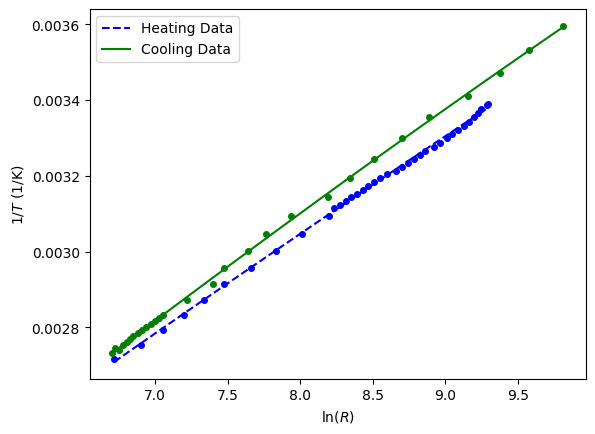
\includegraphics[\textwidth]{Untitled.png}
\caption{Plot of $\ln R$ vs $1/T$}
\end{figure}

\section{Result}

Heating fit parameters: 
\[
\begin{split}
A &= (8.49 \pm 0.07) \times 10^{-4} \\
B &= (2.82 \pm 0.14) \times 10^{-4} \\
C &= (-1.10 \pm 0.70) \times 10^{-7}
\end{split}
\]

Cooling fit parameters: 
\[
\begin{split}
A &= (6.87 \pm 0.08) \times 10^{-4} \\
B &= (3.13 \pm 0.14) \times 10^{-4} \\
C &= (-1.72 \pm 0.74) \times 10^{-7}
\end{split}
\]

\noindent\fbox{%
    \parbox{\textwidth}{%
The thermistor demonstrates sufficient temperature sensitivity for precision measurements. Although observed hysteresis between heating and cooling cycle will require some modification to the theoretical equation to calculate the temperature.
       }%
}\\


\noindent\rule{\linewidth}{0.4pt}
\vspace{2cm}
\bibliography{aipsamp}

\end{document}
